\documentclass{acm_proc_article-sp}
\usepackage{color}
\usepackage{comment}
\usepackage{url}

\newcommand{\bu}[1]{{\color{blue}#1}}
\newcommand{\mm}[1]{{\color{red}#1}}

\begin{document}

\title{Towards Performance Modeling as a Service by Exploiting Resource Diversity in the Public Cloud}

\numberofauthors{2}
\author{
% You can go ahead and credit any number of authors here,
% e.g. one 'row of three' or two rows (consisting of one row of three
% and a second row of one, two or three).
%
% The command \alignauthor (no curly braces needed) should
% precede each author name, affiliation/snail-mail address and
% e-mail address. Additionally, tag each line of
% affiliation/address with \affaddr, and tag the
% e-mail address with \email.
%
% 1st. author
\alignauthor
Mark Meredith\\
       \affaddr{Dept. of Comp. Sci. and Eng.}\\
       \affaddr{The Penn State University}\\
       \affaddr{University Park, PA 16802}\\
       \email{mwm126@gmail.com}
\alignauthor
Bhuvan Urgaonkar\\
       \affaddr{Dept. of Comp. Sci. and Eng.}\\
       \affaddr{The Penn State University}\\
       \affaddr{University Park, PA, 16802}\\
       \email{bhuvan@cse.psu.edu}
}
% There's nothing stopping you putting the seventh, eighth, etc.
% author on the opening page (as the 'third row') but we ask,
% for aesthetic reasons that you place these 'additional authors'
% in the \additional authors block, viz.
%\additionalauthors{Additional authors: John Smith (The Th{\o}rv{\"a}ld Group,
%email: {\texttt{jsmith@affiliation.org}}) and Julius P.~Kumquat
%(The Kumquat Consortium, email: {\texttt{jpkumquat@consortium.net}}).}
%\date{30 July 1999}
% Just remember to make sure that the TOTAL number of authors
% is the number that will appear on the first page PLUS the
% number that will appear in the \additionalauthors section.

\maketitle

%\setcounter{1}
%\pagenumbering{arabic}


\begin{abstract}
%One of the main benefits of virtualization through cloud computing is the ready availability of large rapid virtual machines for rapid application deployment. As computing hardware advances, cloud computing vendors offer new virtual machines with new performance characteristics, adding to the large set of virtual machine types to choose from. Many virtual machine types are available, with varying performance and pricing options. In this work we present a statistical model for estimating the performance of new virtual machine types based on knowledge of existing types. This model is based on data collected by running the Yahoo! Cloud Services Benchmark (YCSB). The databases surveyed are the key-value database Redis, deployed on Amazon Elasticache, and the NoSQL databases Apache Cassandra, deployed on Amazon Elastic Compute Cloud. We tested these on a variety of Amazon virtual machines types.

\end{abstract}

\keywords{Performance modeling, public cloud, regression, empirical evaluation} % NOT required for Proceedings

\section{Introduction}
\vspace{10pt}

%Cloud vendors offer a lot of different virtual machine instance types. Cloud tenants needs to determine what benefit new virtual machine types will bring to their applications.

Many enterprises are migrating their information technology (IT) needs to public cloud computing platforms, a trend that is projected to continue unabated in the foreseeable future~\cite{xxx}. Among the most important reasons behind these ``tenants'' choosing to procure their IT needs from a public cloud is the promise of lower costs. To effectively realize these cost-related benefits, however, it is crucial that these tenants carry out careful dynamic procurement of IT resources to match their evolving needs. Numerous studies show that approaches based on over-provisioning or other ``crude'' estimates of resource needs may negate the cost benefit potential that migrating to a public cloud may offer~\cite{xxx}. Therefore, tenant-side resource procurement has emerged as an area of active research with different aspects of it receiving attention both in academic papers~\cite{xxx} and industrial products~\cite{xxx}. 

Procuring resources cost-effectively from a public cloud provider poses significant technical challenges. One such challenge concerns the problem of determining the set of IT resources (including their capacities) - virtual machines, the virtual network connecting these VMs, storage, etc. - that would be needed to cost-effectively meet the predicted workload of the tenant's software application while offering satisfactory performance and availability to its users. In order to solve this problem, a tenant must first solve the problem of assessing the performance the users of its application software are likely to experience if the application were assigned a given set of IT resources to meet its predicted workload. Our interest in this paper is in this latter problem, often labeled {\it application performance modeling}~\cite{sigmetrics05,xxx}. 

%\noindent{\bf The Problem:} **state the problem.** 

% explain why it is challenging to solve this problem in a public cloud ecosystem
Whereas application performance modeling has been an area of extensive research for many decades across many communities, solving it for the public cloud ecosystem presents a tenant with non-trivial sources of complexity. In particular, most modeling solutions have been developed for traditional private settings and may not be readily adapted to a public cloud. A typical example of such a private setting is a data center or a cluster privately owned and operated by an enterprise that is considering replacing it in favor of a move of its IT needs to a public cloud. 

\begin{figure}[htbp]
\centering
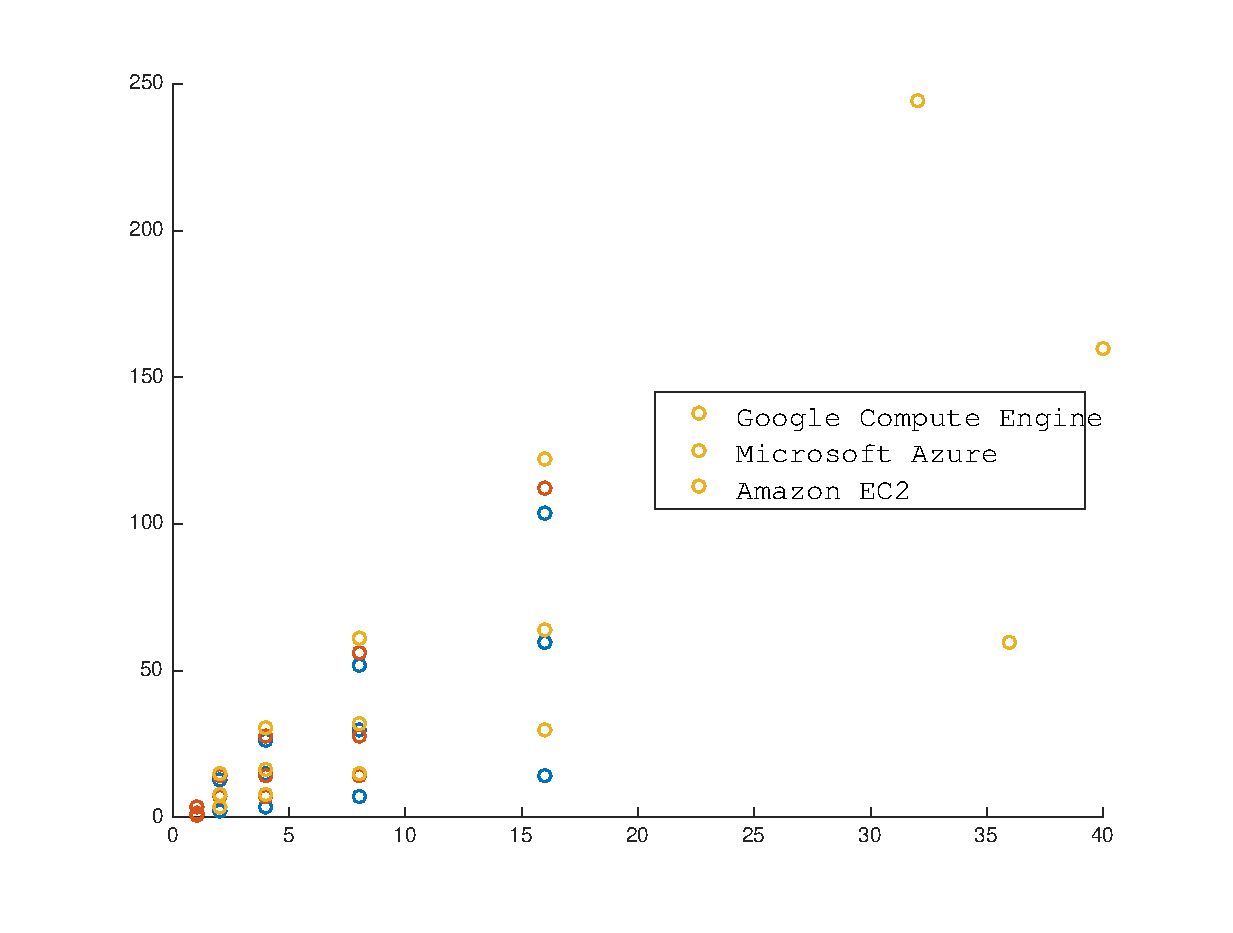
\includegraphics[width=0.45\textwidth]{cloud_vm_types.eps}
\caption{Virtual Machine types available from multiple cloud vendors. 
~\bu{TODO: cleanup plot formatting; make the numbers on the axes larger, label both the axes, use darker colors, move the box with names of providers to the top-left part of the graph.}} \label{fig:diversity}
%\vspace{-10pt}
\end{figure}


Arguably, the most important difference between  these two settings (from the point of view of application performance modeling) is the immense {\it diversity of resources} that a typical public cloud offers.~\footnote{There are other important differences complementary to our focus in this paper and part of our future work. E.g., in a private setting, the user of a machine (tenant application) coincides with its owner while in a public setting the two are separated via virtualization techniques. } We will focus on virtual machines (VMs) as the resource type of interest in this work although our arguments likely apply to other resource types as well. To appreciate this diversity, let us consider some examples from the most prominent public cloud providers that offer many VM types since they need to cater to many different types of customers.  ~\mm{Here virtual machine instance types are organized in groups based on use case.  Instances within a group generally have the same CPU generation and clock speed, and vary by the number of CPUs and memory.  Amazon EC2 offers over 40 VM types organized in eight different groups, varying in CPU, memory, network bandwidth, storage speed, and pricing~\cite{amazon-ec2}. Google Compute Engine offers 15 instance types organized in four groups: Standard, High CPU, High Memory, and Shared Core (for lightweight applications)~\cite{googlecomputeengine}. Finally, Windows Azure ...~\cite{windowsazure}. Figure~\ref{figure:diversity} shows 30 VM instance types organized into four groups: Basic, Standard, Optimized, and Optimized (version 2). ...} 

A typical privately owned data center, on the other hand, is likely to possess a much smaller number of machine types. Keeping machines (and their software configurations) relatively homogeneous brings about significant benefits related to ease of system administration and cost savings (e.g., due to bulk purchase offers from IT vendors). Although factors such as incremental procurement over time, meeting specialized needs (e.g., machines with GPUs), etc.,  do result in some differences among machine types even in a private data center, the overall degree of heterogeneity is significantly smaller than that seen in a  public cloud.

 

This high diversity of resource types in a public cloud introduces an additional source of complexity into a tenant's decision-making. Since the number of resource types in traditional IT environments are small and relatively fixed, performance models have conventionally been developed and calibrated using performance measurements (``profiling'') on the same/similar type of machines on which the application would eventually execute. On the other hand, a tenant of a public cloud would be interested in being able to predict the performance that its workload might experience on a wide variety of resource types that the provider offers. This is because which resource types are the most cost-effective for a tenant's workload might change over time due to: (i) changes in the tenant's own workload (e.g., many applications show periodic time-of-day or seasonal variations in their workload intensities) and (ii) dynamism and variety in the cloud provider's pricing schemes (e.g., Amazon EC2 offers spot pricing for most of its instance types and such spot instances are usually much cheaper than their on-demand counterparts). Clearly, approaches based on calibrating a tenant's performance models separately on the dozens of resource types that public clouds offer are likely to not be scalable. Additionally, such approaches may prove to be expensive. 

% introduce the idea of exploiting diversity instead of letting it be a hindrance. 
We wish to explore if a tenant {\em might actually be able to benefit from this diversity} by delibearately and carefully exploiting it to ease the creation and calibration of effective performance models. *** explain why we expect this to be the case. ***

\noindent{\bf The Hypothesis:} Diversity of VMs in a public cloud can aid in the calibration of tenant application performance models on unseen VMs. 

An important aspect of our hypothesis worth highlighting is that it is not tied to a specific performance modeling approach. ** expand this **

\noindent {\bf Our Approach and Contributions:} In this paper, we take a small first step towards exploring the above idea. Specifically, we devise a multi-linear regression modeling framework for predicting the performance of interactive data storage server applications. We calibrate this model for three different types of real-world applications: (i) Redis, a ..., (ii) Apache Cassandra, a ..., (iii) Mysql, a popular open-source ACID database. We ... 

Our key findings are as follows:
\begin{itemize}
\item ...
\item ...
\item ...
\end{itemize}


To the best of our knowledge, ... On the one hand, our work is highly complementary to traditional performance modeling research. At the same time, it opens up a promising new area for further research. As part of our own future work, we plan to ... ** discuss the possibility of offering PMaaS as a key implication of our work as well as being an interesting direction for future research. **

The rest of this paper is organized as follows. In Section~\ref{sec:back}, we present some background material.  In Section~\ref{sec:model}, we describe the performance modeling techniques that we employ.  In Section~\ref{sec:eval}, we present our empirical evaluation of our hypothesis using three real-world applications as our case studies. We discuss related work in Section~\ref{sec:related}.  Finally, we discuss unresolved challenges and future directions in Section~\ref{sec:future} and conclude in Section~\ref{sec:conclus}. 


%Solution: test your application on different VM types and find out?

%present the problem, its significance, and key challenges
 
%explain why the state-of-the-art may not be adequate, particularly as clouds move towards higher levels of utilization and dynamism

%explain our key ideas and contributions

\section{Background}
\label{sec:back}
\vspace{10pt}

%big picture overview of tenant-side decision-making, where PMaaS fits within this, mention the specific assumptions we make, the chosen environment, which ideas are likely to generalize to other settings
 
\begin{figure*}%[htbp]
\centering
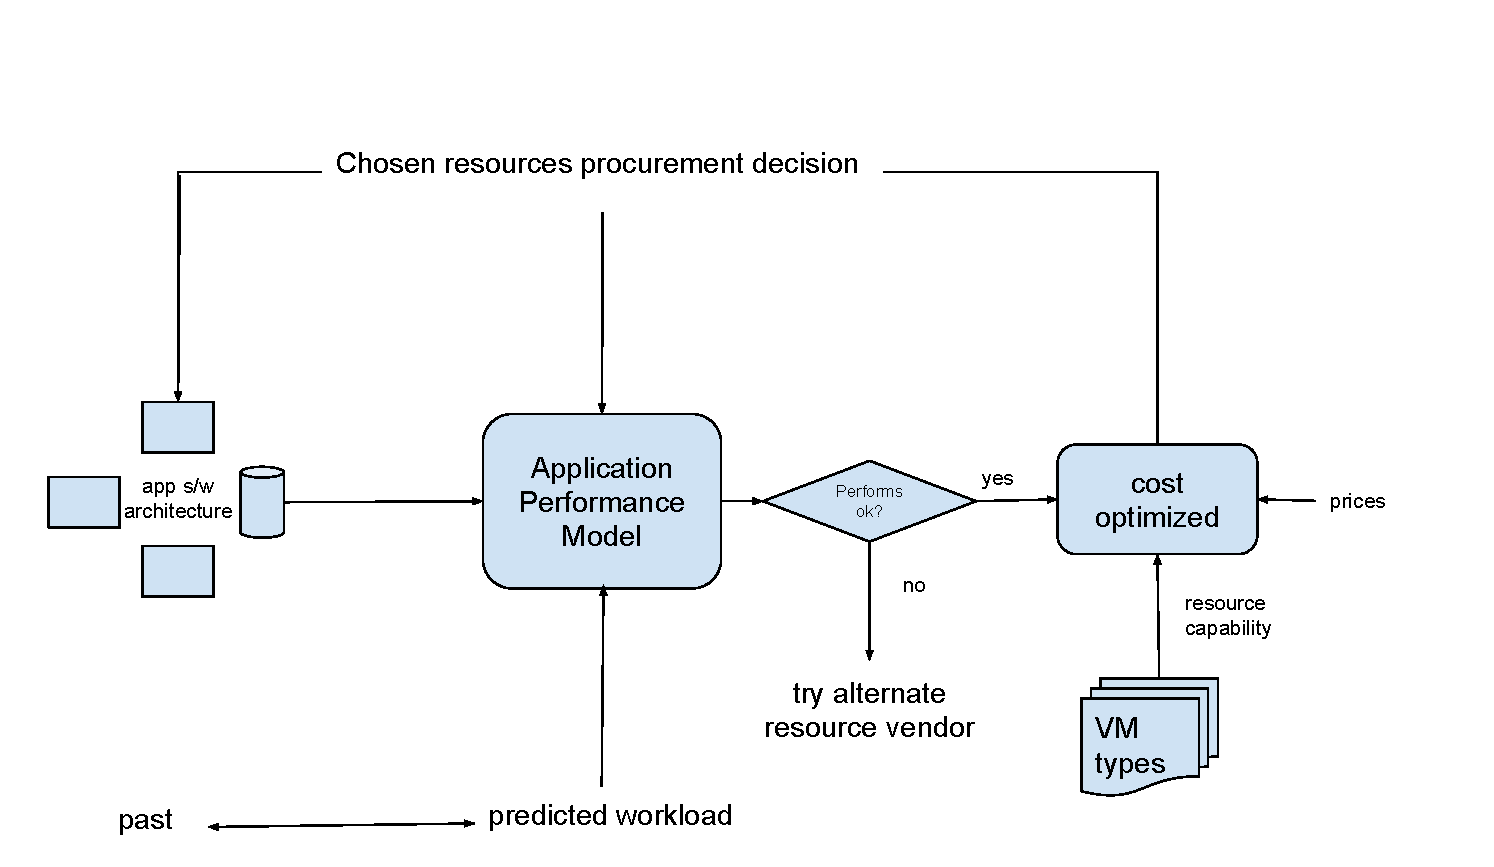
\includegraphics[width=0.8\textwidth]{pmass_diagram}
\caption{An overview of interaction between the performance modeling problem we study and other aspects of decision-making for a cost-conscious tenant procuring resources from a public cloud. ~\bu{TODO: Improve this figure. Can discuss on Tuesday morning.}} 
\label{fig:diagram}
%\vspace{-10pt}
\end{figure*}

Figure~\ref{fig:diagram} shows the essential elements making up the decision-making that a general cost-conscious tenant might carry out for procuring resources from a public cloud. In particular, it clarifies the role of application performance modeling within this overall decision-making and its interaction with other elements. 
%** expand this, 
The tenant would employ observations of its workload intensity in the past to predict its future workload. Whereas some tenants exhibit significant predictability (e.g., captured well via Markovian models)~\cite{xxx}, others are known to exhibit poor predictability and must resort to short-term (``myopic'') estimates~\cite{xxx}. Regardless, having made these predictions, the tenant must then ascertain the VMs to add to (or deallocate from) its resource pool. 

Figure~\ref{fig:diagram} shows one way of thinking about this decision-making, wherein the tenant determines (using its application performance model) resource allocation choices that would allow it to meet its predicted workload with the requisite performance goals. These choices are then compared in terms of their costs (or expected profits) via an optimization problem that incororates idiosyncrasies of the prices offered by the public cloud.~\footnote{The actual realization of the overall decision-making may be different from how we describe it here. Our description is deliberately designed to highlight the role of the application performance model.} 

**point to related work, repeat that our arguments are not tied to a particular modeling technique. **

%what about the costs of PMaaS itself? how to make it practical? might providers actually offer it as a service?

\section{Our Modeling Methodology}
\label{sec:model}
\vspace{10pt}
In this section, we describe the general regression-based performance modeling ideas we employ in our research. In Section~\ref{sec:eval}, we describe how we adapt this basic model to our 3 application case studies whose performance we study on the Amazon EC2 cloud. 

%\subsection{Methodology}
%\vspace{10pt}



\mm{
Our goal is to model the performance of different cloud virtual machine instance types for different applications, and show a correlation between the performance of those applications that can predict the performance of those applications on new virtual machine instance types.

For server applications, the performance can be characterized by throughput (request per second) and latency (duration of each request).  For low rates of throughput, the latency is nearly constant and increases slowly with increasing throughput.  As throughput approaches the maximum capacity of the server, the latency increases much more rapidly.  (Add Figure ???) For our study, we study the low-throughput region, which is approximately linear for a variety of VM instances, applications, and throughputs.

We did a multilinear regression with the latency as the dependent variable and dependent variables throughput, CPU count, and memory.  The regression uses the data for a set of instances we call the "training set".

We use the regression to predict the performance for another virtual machine type (the "test instance") outside of the training set.

As the number of virtual machine instances in the training set increases, the fit for the test instance improves.

We used the Amazon EC2 virtual machine instances listed in Table \label{table:awstypes}.  There are three instances from the M3 group (standard) and three from the R3 group (memory optimized).  The memory/cpu ratio is the same within each group, with the R3 group having twice the memory/cpu as the M3 group.  This is necessary for the CPUs and memory to be independent variables in the regression.

\begin{itemize}
\item multiple linear regression on data for 3 VM types
\item use model to get predicted residuals for 1 VM type
\item add data for other VM types to the model
\item note that the residual decreases when fitting model to more terms
\end{itemize}

}

%\subsection{Predictive Residual}
%\vspace{10pt}

We evaluate the goodness of fit of the model for each training set with the Predictive Residual, $R^2_{predicted}$.

For multiple linear regressions, the coefficient of determination $R^2$ always increases when adding independent variables.  A better measure of goodness of fit is for our model is predicted $R^2$, defined in terms of PRESS statistic, which in turn is defined in terms of

We do a multiple linear regression on the parameters in Table XXX for the data from a set of VM instance types to get a linear regression model $y_i = \beta_1 x_i1+\dotfill+\beta_{p}x_{ip}$

We use the model to find predicted values for the test instance type.

As more VM instances are added to training data, the model fits better for predicting values for the test instance type.  The goodness of fit is defined as the normalized residual:

\newdef{definition}{Definition}
\begin{definition}
Predicted Residual
\begin{displaymath}{
Predicted Residual=\sum_{i=1}^{n} (y_i - \hat{y}(x_i))^{2}
}\end{displaymath}

\end{definition}

The residual is normalized with the total sum of squares for the test data from the mean.

\begin{definition}
TSS (Total Sum of Squares)
\begin{displaymath}{
TSS=\sum_{i=1}^{n} (y_i - \bar{y})^{2}
}\end{displaymath}

\begin{displaymath}{
R_{predicted}^2 = (1 - PredictedResidual/TSS)
}\end{displaymath}
\end{definition}

\section{Evaluation}
\label{sec:eval}
\vspace{10pt}

\subsection{Methodology and Setup}
\vspace{10pt}

\begin{table}
\centering

\begin{tabular}{|r|l|c|r|l|} \hline
Instance name & Abbr.& \# cores&Memory&Network\\ \hline
r3.large & $VM_1$ & 2 & 15 GB & Moderate\\ \hline
r3.xlarge & $VM_2$ & 4 & 30.5 GB & Moderate\\ \hline
r3.2xlarge & $VM_3$ & 8 & 61 GB & High\\ \hline
m3.large & $VM_4$ & 2 & 7.5 GB & Moderate\\ \hline
m3.xlarge & $VM_5$ & 4 & 15 GB & Moderate\\ \hline
m3.2xlarge & $VM_6$ & 8 & 30 GB & High\\ \hline
\hline\end{tabular}
\caption{AWS instance types employed in our evaluation. }
\label{table:awstypes}
\end{table}


\mm{
We benchmarked virtual machines on the most widely used cloud vendor, Amazon Web Services (AWS).

We studied three different types of databases: Apache Cassandra (NoSQL database), Redis (Key-Value caching database), and MySQL (SQL database).

For benchmarking we used the open-source Yahoo! Cloud Serving Benchmark (YCSB).  For each test case we loaded the database with 1000000 records, each containing ten fields of 100 bytes each (the default).  YCSB defines several standard workloads; we used Workload B (95\% read 5\% write).  The requests for records were made using the zipfian probability distribution.

We ran the YCSB client on a m4.2xlarge EC2 instance running Ubuntu Linux 14.04. We monitored the system load average on the client machine to verify that the client was not the bottleneck during the tests.
}

\subsection{Case Study 1: Redis}
\vspace{10pt}

\mm{
Redis is an open-source, key/value NoSQL database.  Redis is in-memory, and therefore very fast-durability is optional, so Redis can be used either as a primary or caching database.

Redis was deployed on AWS using Amazon ElastiCache, a web service that abstracts the deployment and administration of the OS and database software.  Elasticache supports up to five read replicas of the primary database.  For our testing we only used a single instance.

We used VM type r3.2xlarge as test data, while increasing the training data in Table \ref{table:redis} and Figure \ref{figure:redisbarread}.  The fit improves as more VMs are added to the training set, as shown in Figure \ref{figure:redisread} and Figure \ref{figure:rediswrite}.
}

% \begin{table}
% \centering
% \caption{Redis $R_{predicted}^2$ for $VM_6$}
% \begin{tabular}{|r|r|l|} \hline
% $R_{read}^2$&$R_{write}^2$&Training Data\\ \hline
% -0.657113 & -0.573816 & $VM_1$\\ \hline
% 0.155888 & 0.0674494 & $VM_1,VM_2$\\ \hline
% 0.43653 & 0.395256 & $VM_1,VM_2,VM_3$\\ \hline
% 0.783798 & 0.727331 & $VM_1,VM_2,VM_3,VM_4$\\ \hline
% 0.80571 & 0.748588 & $VM_1,VM_2,VM_3,VM_4,VM_5$\\ \hline
% %0.86354 & 0.836441 & $VM_1,VM_2,VM_3,V_4,V_5,V_6$\\ \hline
% \hline\end{tabular}
% \label{table:redis}
% \end{table}



\begin{table}
\centering
\caption{Redis $R_{predicted}^2$ for $VM_6$}
\begin{tabular}{|r|r|l|} \hline
$R_{read}^2$&$R_{write}^2$&Training Data\\ \hline
-0.648416 & -1.12245 & VM6 \\ \hline 
0.51488 & 0.547705 & VM6 VM5 \\ \hline 
0.738979 & 0.738969 & VM6 VM5 VM3 \\ \hline 
0.832156 & 0.821984 & VM6 VM5 VM3 VM1 \\ \hline 
0.837957 & 0.827944 & VM6 VM5 VM3 VM1 VM4 \\ \hline 
\hline\end{tabular}
\label{table:redis}
\end{table}

\begin{table}
\centering
\caption{Redis $R_{predicted}^2$ for $VM_6$}
\begin{tabular}{|r|r|l|} \hline
$R_{read}^2$&$R_{write}^2$&Training Data\\ \hline
-0.648416 & -1.12245 & VM6 \\ \hline 
0.506158 & 0.41527 & VM6 VM3 \\ \hline 
0.738979 & 0.738969 & VM6 VM3 VM5 \\ \hline 
0.776002 & 0.756578 & VM6 VM3 VM5 VM4 \\ \hline 
0.837957 & 0.827944 & VM6 VM3 VM5 VM4 VM1 \\ \hline 
\hline\end{tabular}
\label{table:redis}
\end{table}

\begin{table}
\centering
\caption{Redis $R_{predicted}^2$ for $VM_6$}
\begin{tabular}{|r|r|l|} \hline
$R_{read}^2$&$R_{write}^2$&Training Data\\ \hline
-0.559516 & -0.47657 & VM5 \\ \hline 
0.51488 & 0.547705 & VM5 VM6 \\ \hline 
0.738979 & 0.738969 & VM5 VM6 VM3 \\ \hline 
0.776002 & 0.756578 & VM5 VM6 VM3 VM4 \\ \hline 
0.837957 & 0.827944 & VM5 VM6 VM3 VM4 VM1 \\ \hline 
\hline\end{tabular}
\label{table:redis}
\end{table}

\begin{table}
\centering
\caption{Redis $R_{predicted}^2$ for $VM_6$}
\begin{tabular}{|r|r|l|} \hline
$R_{read}^2$&$R_{write}^2$&Training Data\\ \hline
-0.559516 & -0.47657 & VM5 \\ \hline 
0.260701 & 0.29636 & VM5 VM3 \\ \hline 
0.738979 & 0.738969 & VM5 VM3 VM6 \\ \hline 
0.776002 & 0.756578 & VM5 VM3 VM6 VM4 \\ \hline 
0.837957 & 0.827944 & VM5 VM3 VM6 VM4 VM1 \\ \hline 
\hline\end{tabular}
\label{table:redis}
\end{table}


  \begin{figure}
    \centering
    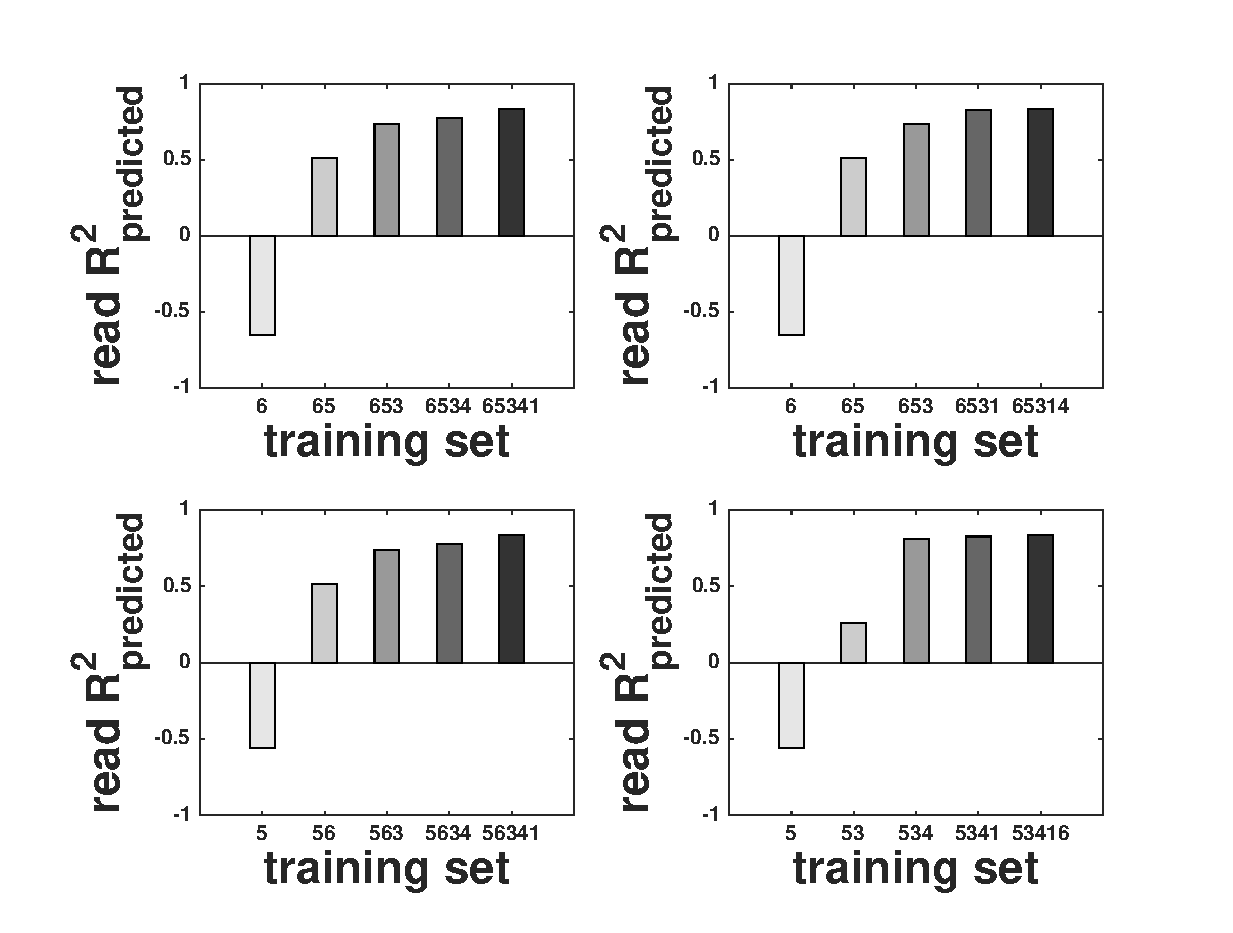
\includegraphics[scale = 0.5]{bar_read_avg_latency.eps}
    \caption{Redis read R-squared vs training set}
    \label{figure:redisbarread}
  \end{figure}

  \begin{figure}
    \centering
    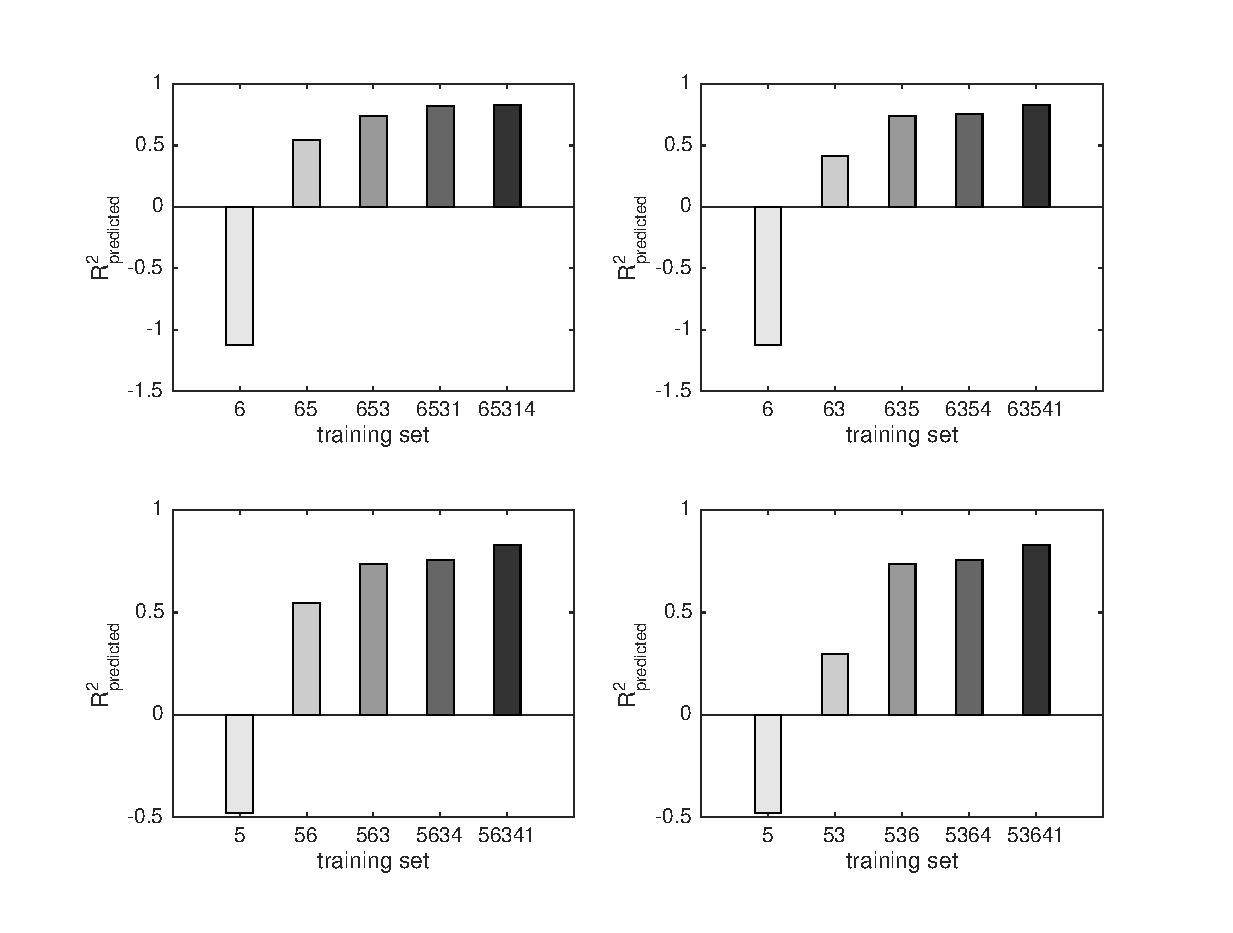
\includegraphics[scale = 0.5]{bar_write_avg_latency.eps}
    \caption{Redis write R-squared vs training set}
    \label{figure:redisbarread}
  \end{figure}

  \begin{figure}
\centering
\begin{minipage}{.25\textwidth}
  \centering
    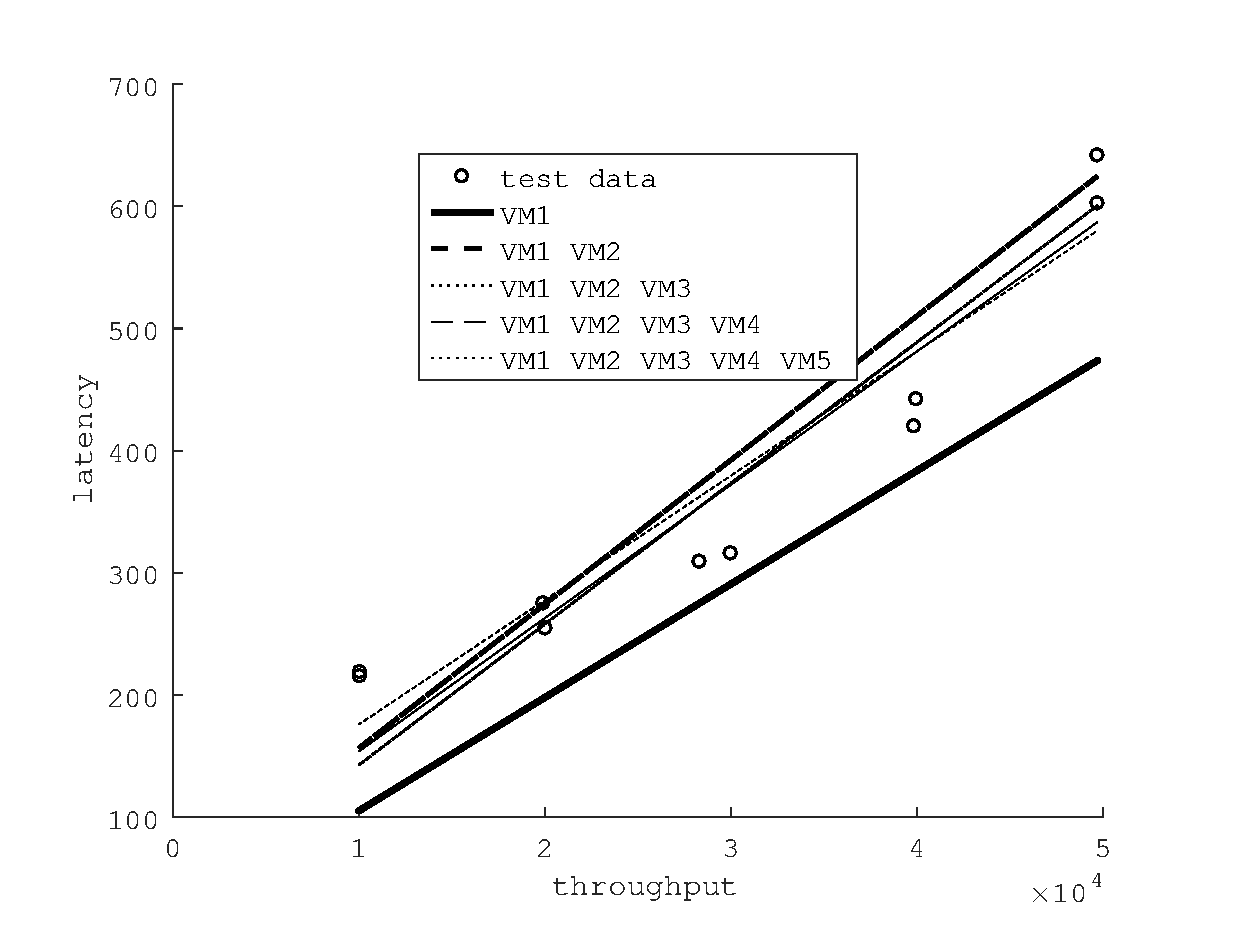
\includegraphics[scale = 0.25]{fit_write_avg_latency_r3_2x_r3__m3_2x_m3__r3_x_m3_x.eps}
    \caption{Redis average write latency vs throughput}
    \label{figure:redisbarread}
\end{minipage}%
\begin{minipage}{.25\textwidth}
  \centering
    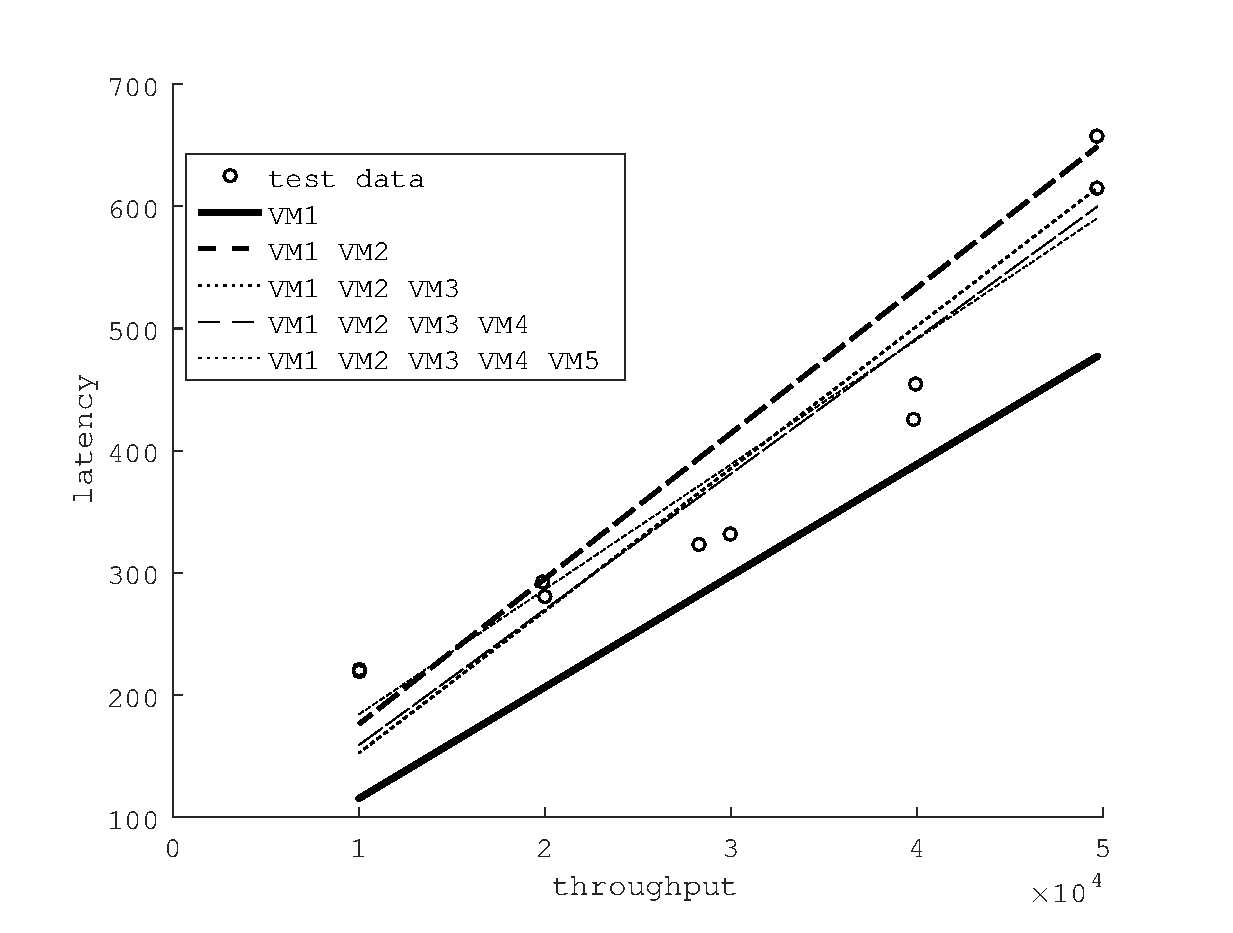
\includegraphics[scale = 0.25]{fit_read_avg_latency_r3_2x_r3__m3_2x_m3__r3_x_m3_x.eps}
    \caption{Redis average read latency vs throughput}
  \label{fig:redisbarread}
\end{minipage}
  \end{figure}

\subsection{Case Study 2: Apache Cassandra}
\vspace{10pt}

\mm{
Apache Cassandra is a Table/Key-Value hybrid NoSQL database.  It is suitable for applications that require high availability provided by replication.

Apache Cassandra was installed on Amazon EC2 instances of various VM instance types.  Our testing was done on Cassandra clusters with 5 nodes.

\begin{itemize}
   \item present linear regression model, explain simplifications, justifications
   \item present non-linear regression model if applicable
\end{itemize}

\subsubsection{Evaluation for a Strict Consistency Configuration}

\begin{itemize}
\item replication factor=3 (crashes for >1)
\item consistency N/A (ONE==ALL)
\end{itemize}
Workload B (95/5 r/w) with uniform distribution

Present data for
7 gen VM types, 3 workloads, 1-5 nodes, replication factor 1

  \begin{figure}
    \centering
    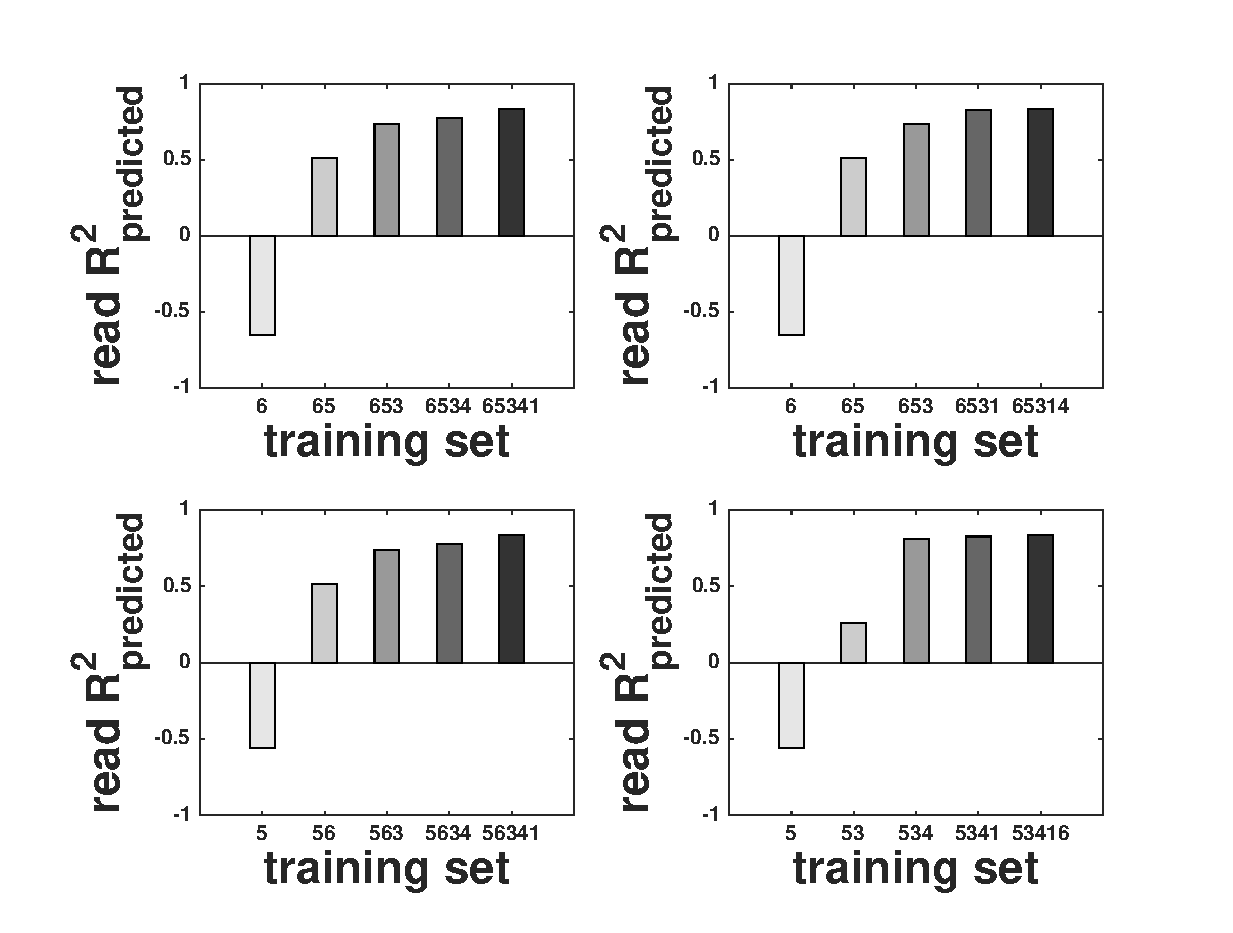
\includegraphics[scale = 0.5]{bar_read_avg_latency.eps}
    \caption{Cassandra read R-squared vs training set TODO: copy-pasted from Redis as placeholder}
    \label{figure:redisbarread}
  \end{figure}

  \begin{figure}
    \centering
    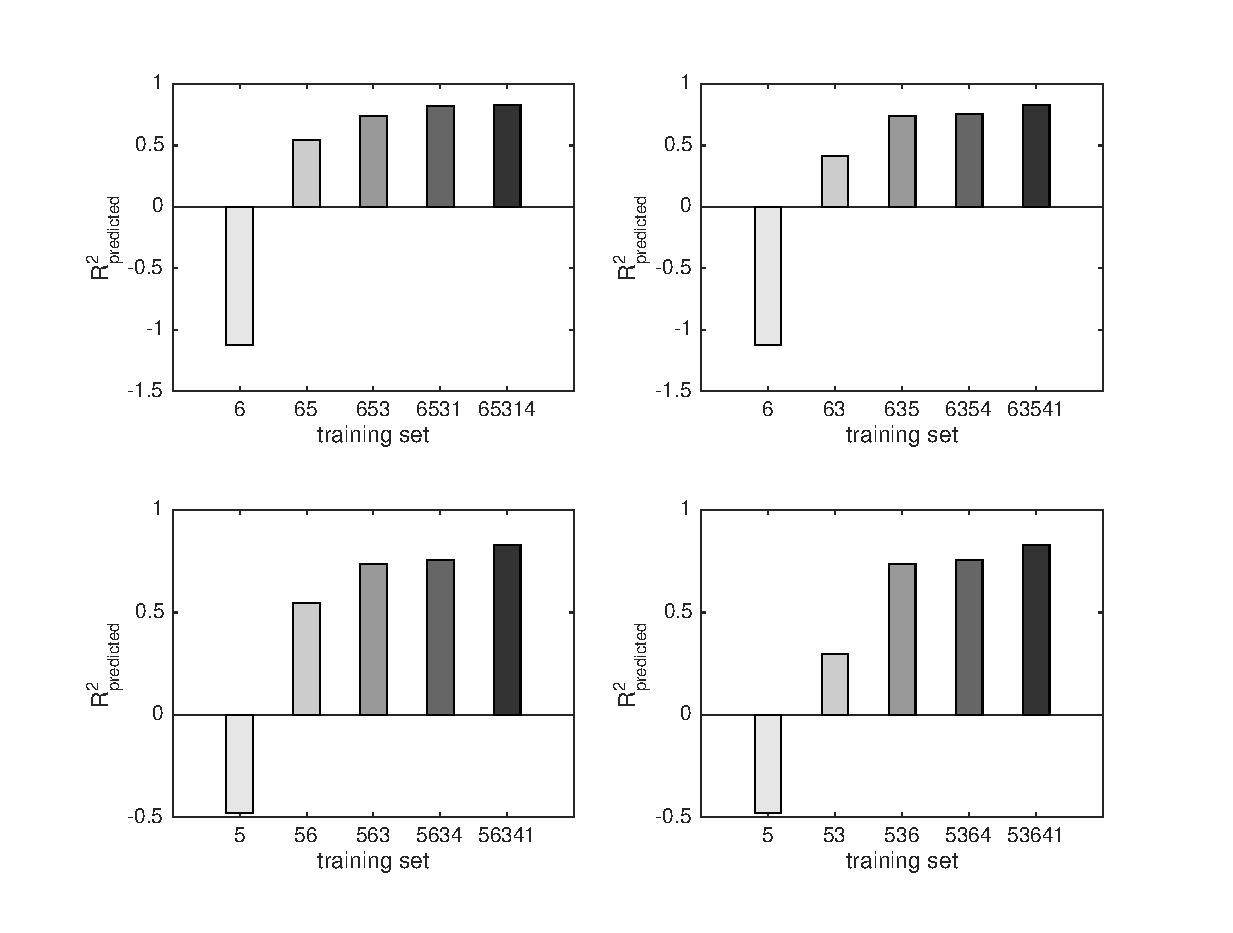
\includegraphics[scale = 0.5]{bar_write_avg_latency.eps}
    \caption{Cassandra write R-squared vs training set TODO: copy-pasted from Redis as placeholder}
    \label{figure:redisbarread}
  \end{figure}

% \subsubsection{Evaluation for a Weak Consistency Configuration}

% consistency=ONE

% Workload B (95/5 r/w) with uniform distribution

% Present data for
% 3 VM types: gen,mem,cpu, throughputs 5000-20000, replication factor 3, 5 nodes
}
\subsection{MySQL}
\vspace{10pt}

\mm{
MySQL was deployed using Amazon Relational Database Service (Amazon RDS), which abstracts away the deployment and administration of OS and relationship database software.

MySQL was deployed to six VM types as listed in Table \ref{table:rdstypes}.

We tested using YCSB Workload A (50\% read, 50\% write) with a uniform distribution.

We did a multiple linear regression on the variables throughput, cores, memory, and network.  (Network performance was quantified by representing it as an dummy variable.)

We used VM type r3.2xlarge as test data, while increasing the training data in Table \ref{table:mysql}.

However, the data for MySQL did not fit a multilinear regression well.  This may be due to the higher write latency of SQL databases, or something with Amazon's RDS architecture that made our YCSB testing method unsuitable.  Another possibility is that the network availability varied over time with RDS, making data collection unrepeatable.
}

\begin{table}
\centering
\caption{MySQL $R_{predicted}^2$ for $VM_6$}
\begin{tabular}{|r|r|l|} \hline
$R_{read}^2$&$R_{write}^2$&Training Data\\ \hline
0 & 0& $VM_1,VM_2,VM_3$\\ \hline
0 & 0& $VM_1,VM_2,VM_3,VM_4$\\ \hline
0 & 0& $VM_1,VM_2,VM_3,V_4,V_5$\\ \hline
\hline\end{tabular}
\label{table:mysql}
\end{table}

\section{Related Work}
\label{sec:related}
\vspace{10pt}

\begin{itemize}
   \item Chris Stewart - non-stationarity of workloads
   \item Delta modeling from CMU
   \item Graybox modeling from Wisconsin
   \item work by Shivnath Babu of Duke
\end{itemize}


\section{Lessons, Challenges, and Future Directions}
\label{sec:future}
\vspace{10pt}

what about the costs of PMaaS itself? how to make it practical? might providers actually offer it as a service?

\section{Conclusions}
\label{sec:conclus}
\vspace{10pt}

%\end{document}  % This is where a 'short' article might terminate


%
% The following two commands are all you need in the
% initial runs of your .tex file to
% produce the bibliography for the citations in your paper.
\bibliographystyle{abbrv}
\bibliography{refs.bib}  % sigproc.bib is the name of the Bibliography in this case
% You must have a proper ".bib" file
%  and remember to run:
% latex bibtex latex latex
% to resolve all references
%
% ACM needs 'a single self-contained file'!
%

\balancecolumns
% That's all folks!
\end{document}
